%___________________________________________
%*************************************************************
% Existing Work
%___________________________________________
%^^^^^^^^^^^^^^^^^^^^^^^^^^^^^^^^^^^^^^^^^^^^^^^^^^^

\section{Existing Work}

%-----------------------------------------------------------------------
% Learning in Games (Current Work in Field)
%-----------------------------------------------------------------------

\subsection{Learning Agents and Game AI Competitions}
\label{subsec:gameaicomps}

Over the last few years several game based AI competitions have been run, over a variety of genres. These competitions challenge entrants to implement an agent that plays a game and is rated according to the competitions specification. They have attracted both academic \cite[p.~2]{2012the} and media interest \cite[p.~2]{marioaicomp}. The competition tend to encourage the use of learning techniques. Hence, several interesting papers concerning the application of biologically inspired learning agents in video games have recently been published. Approaches tend to vary widely, modelling and tackling the problem very differently and specialising techniques in previously unseen ways. \cite[p.~11]{2012the}

Some brief details of the competitions which are of relevance to this project are compiled in to Table \ref{tab:gameaicomp}. The Mario AI Competition is also explored in more detail below.

\begin{table}
  \begin{adjustwidth}{-4cm}{-4cm}
  \begin{center} \small
    \begin{tabular}{ | >{\raggedright}p{2cm} | >{\raggedright}p{2cm} | p{7.5cm} |}
    \hline
    \textbf{Genre} & \textbf{Game} & \textbf{Description} \TBstrut \\ \thickhline
    Racing & TORCS (Open-source) \cite{torcs} &  
    \textbf{The Simulated Car Racing Competition}\newline Competitors enter agent drivers, that undergo races against other entrants which include qualifying and multi-car racing. The competition encourages the use of learning techniques. \cite{scrc}
      \\ \hline
    First Person Shooter (FPS) & Unreal Tournament 2004 &
    \textbf{The 2K BotPrize}\newline Competitors enter `bots' that play a multi-player game against a mix of other bots and humans. Entrants are judged on Turing test basis, where a panel of judges attempt to identify the human players. \cite{2kbot}
       \\ \hline
    Real Time Strategy (RTS) & Starcraft &
    \textbf{The Starcraft AI Competition}\newline Agents play against each other in a 1 on 1 knockout style tournament. Implementing an agent involves solving both micro objectives, such as path-planning, and macro objectives, such as base progression. \cite{starcomp}
       \\ \hline
    Platformer & Infinite Mario Bros (Open-source) &
    \textbf{The Mario AI Competition}\newline Competitors submit agents that attempt to play (as a human would) or create levels. The competition is split into `tracks', including Gameplay, Learning, Turing and Level Generation. In Gameplay, each agent must play unseen levels, earning a score, which is compared to other entrants. \cite{2012the} 
       \\ \hline
    
    \end{tabular}
  \end{center}
  \end{adjustwidth}
  \caption{\small This table summarises some recent game AI competitions \cite{2014how}}
  \label{tab:gameaicomp}
\end{table}

\subsubsection{The Mario AI Competition}
\label{subsec:marioaibench}

The Mario AI Competition, organised by Sergey Karakovskiy and Julian Togelius, ran between 2009-2012 and used an adapted version of the open-source game Infinite Mario Bros. From 2010 onwards the competition was split into four distinct `tracks'. We shall focus on the unseen Gameplay track, where agents play several unseen levels as Mario with the aim to finish the level (and score highly). \cite{marioaicomp} \cite{2012the}

\subsubsection*{\hspace{6pt}Infinite Mario Bros.}

Infinite Mario Bros (IMB) \cite{imb} is an open-source clone of Super Mario Bros.~3, created by Markus Persson. The core gameplay is described as a \emph{Platformer}. The game is viewed side-on with a 2D perspective. Players control Mario and travel left to right in an attempt to reach the end of the level (and maximise score). The screen shows a short section of the level, with Mario centred. Mario must navigating terrain and avoid enemies and pits. To do this Mario can move left and right, jump, duck and speed up. Mario also exists in 3 different states, \emph{small}, \emph{big} and \emph{fire} (the latter of which enables Mario to shoot fireballs), accessed by finding powerups. Touching an enemy (in most cases) reverts Mario to a previous state. Mario dies if he touches an enemy in the \emph{small} state or falls into a pit, at which point the level ends. Score is affected by how many coins Mario has collected, how many enemies he has killed (by jumping on them or by using fireballs or shells) and how quickly he has completed the level. \cite[p.~3]{2012the}

An example of a typical level in IMB can be found in Figure \ref{fig:xmpllevel}.

\subsubsection*{\hspace{6pt}Suitability to Learning}

\begin{figure}[t]
	\begin{adjustwidth}{-0cm}{-0cm}
    \centering
    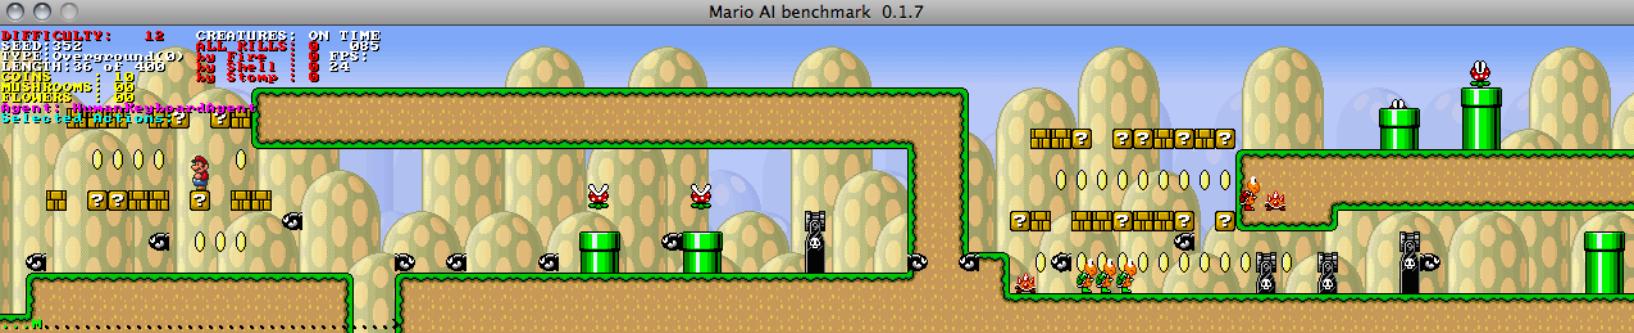
\includegraphics[width=\textwidth]{examplelevel.png}
    \caption{Example of part of a level in the Mario AI Competition's benchmark software. Taken from \cite[p.~6]{2012the}}
    \label{fig:xmpllevel}
    \end{adjustwidth}
\end{figure}

The competitions adaptation of IMB (known henceforth as the `benchmark') incorporates a parameterised level generator and allows for the game to be sped-up by removing the reliance on the GUI and system clock. This makes it a great testbed for reinforcement learning. The ability to learn from large sets of diverse data makes learning a much more effective technique. \cite[p.~3]{2012the}

Besides that, the Mario benchmark presents an interesting challenge for learning algorithms. Despite only a limited view of the ``world" at any one time the state and observable space is still of quite high-dimension. Though not to the same extent, so too is the action space. Any combination of five key presses per timestep gives an action space of $2^5$ \cite[p.~3]{2012the}. Hence part of the problem when implementing a learning algorithm for the Mario benchmark is reducing these search spaces. This has the topic of papers by Handa and Ross and Bagnell \cite{rossbagnell} separately addressed this issue in their papers \cite{handa} and \cite{rossbagnell} respectively.

Lastly, there is a considerable learning curve associated with Mario. The simplest levels could easily be solved by agents hard coded to jump when they reach an obstruction, whereas difficult levels require complex and varied behaviour. For example, traversing a series of pits may require a well placed series of jumps, or passing a group of enemies may require careful timing. Furthermore, considerations such as score, or the need to backtrack from a dead-end greatly increase the complexity of the problem. \cite[p.~3, p.~12]{2012the}


%-----------------------------------------------------------------------
% Previous Agents
%-----------------------------------------------------------------------

\subsection{Previous Learning Agent Approaches}
\label{ssec:prevagents}

Agent-based AI approaches in commercial games tend to focus on finite state machines, behaviour trees and rulesets, with no learning component. Learning agents are more prevalent in AI competitions and academia, where it is not only encouraged, but viewed as an interesting research topic \cite[p.~1]{marioaicomp}. Examples from both standpoints are compiled in Table \ref{tab:agents}.

\subsubsection{Evolutionary Algorithms}

In Section \ref{subsec:concepts} we presented some basic concepts of evolutionary and genetic computing. This approach is a common choice of learning methods used in game-playing agents. D. Perez et al. note in their paper \cite[p.~1]{gramev} that evolutionary algorithms are particularly suitable for video game environments: 
\begin{quote}\itshape
`Their stochastic nature, along with tunable high- or low-level representations, contribute to the discovery of non-obvious solutions, while their population-based nature can contribute to adaptability, particularly in dynamic environments.'
\end{quote}
The evolutionary approach has been used across several genres of video games. For example, \emph{neuroevolution}, a technique that evolves neural networks, was used in both a racing game agent (by L. Cardamone \cite[p.~137]{scrc}) and a FPS agent (by the UT$\wedge$2 team \cite{2kbot}). Perhaps the most popular approach was to use genetic algorithms (GAs) to evolve a more traditional game AI agent. R. Small used a GA to evolve a ruleset for a FPS agent \cite{agentsmith}, T. Sandberg evolved parameters of a potential field in his Starcraft agent \cite{emapf} , \emph{City Conquest's} in-game AI used an agent-based GA-evolved build plan \cite{evolutioningamedesign} and D. Perez et al. used a grammatical evolution (a GA variant) to produce behaviour trees for a Mario AI Competition entry \cite{gramev}.

\subsubsection{Multi-tiered Approaches}

Several of the most successful learning agents take a multi-tiered approach. By splitting high-level behaviour from low-level actions agents can demonstrate a more interesting, and even human-like, performance. For example, COBOSTAR, an entrant in the 2009 Simulated Car Racing Competition, used offline learning to determine high-level parameters such as desired speed and angle alongside a low-level crash avoidance module \cite[p.~136]{scrc}. UT$\wedge$2 used learning to give their FPS bot broad human behaviours and a separate constraint system to limit aiming ability \cite{2kbot}.  Overmind, the winner of the 2010 Starcraft Competition, planned resource use and technology progression at a macro level, but used A* search micro-controllers to coordinate units \cite{overmind}. 

\vspace{\baselineskip} \noindent
One learning agent that successfully utilised both an evolutionary algorithm and a multi-tiered approach is the Mario agent REALM, which is explored in more detail below. 

\subsubsection{REALM}
\label{ssec:realm}

The REALM agent, developed by Slawomir Bojarski and Clare Bates Congdon, was the winner of the 2010 Mario AI competition, in both the unseen and learning Gameplay tracks. REALM stands for \textbf{R}ule Based \textbf{E}volutionary Computation \textbf{A}gent that \textbf{L}earns to Play \textbf{M}ario. REALM went through two versions (V1 and V2), with the second being the agent submitted to the 2010 competition.

\subsubsection*{\hspace{6pt}Rule-based}

Each time step REALM creates a list of binary observations of the current scene, for example {\footnotesize IS\_ENEMY\_CLOSE\_LOWER\_RIGHT} and {\footnotesize IS\_PIT\_AHEAD}. Conditions on observations are mapped to actions in a simple ruleset. These conditions are ternary (either {\footnotesize TRUE}, {\footnotesize FALSE} or {\footnotesize DONT\_CARE}) \cite[p.~85]{realm}. A rule is chosen that best fits the current observations, with ties being settled by rule order, and an action is returned \cite[p.~86]{realm}.

Actions in V1 are explicit key-press combinations, whereas in V2 they are high-level plans. These plans are passed to a simulator, which reassesses the environment and uses A* to produce the key-press combination. This two-tier approach was designed in part to reduce the search space of the learning algorithm. \cite[pp.~85-87]{realm}

\subsubsection*{\hspace{6pt}Learning}

REALM evolves ruleset using an ES for 1000 generations. The best performing rule set from the final generation was chosen to act as the agent for the competition. Hence, REALM is an agent focused on offline learning. \cite[pp.~87-89]{realm}

Populations have a fixed size of 50 individuals, with each individual's genome being a ruleset. Each rule represents a gene and each individual has 20. Initially rules are randomised, with each condition having a 30\%, 30\%, 40\% chance to be {\footnotesize TRUE}, {\footnotesize FALSE} or {\footnotesize DONT\_CARE} respectively.

Individuals are evaluated by running through 12 different levels. The fitness of an individual is a modified score, averaged over the levels. Score focuses on distance, completion of level, Mario's state at the end and number of kills. Each level an individual plays increases in difficulty. Levels are predictably generated, with the seed being recalculated at the start of each generation. This is to avoid over-fitting and to encourage more general rules.

REALM used the $\pmb{(\mu  + \lambda)}$ variant ES, with $\mu = 5$ and $\lambda = 45$ (i.e. the best 5 individuals are chosen and produce 9 clones each). Offspring are exposed to: \textbf{Mutation}, where rule conditions and actions may change value; \textbf{Crossover}, where a rule from one child may be swapped with a rule from another child\footnote{This is similar to a  $\pmb{(\mu/\rho  + \lambda)}$ ES approach with $\rho = 2$, but crossover occurs in the mutation phase and between all children, rather than specifically with children from another parent.} and \textbf{Reordering}, where rules are randomly reordered. These occur with probabilities of 10\%, 10\% and 20\% respectively \cite[p.~88]{realm}. Unfortunately, the method employed to perform these operations is not clearly explained in the REALM paper \cite{realm}.

\subsubsection*{\hspace{6pt}Performance}

The REALM V1 agent saw a larger improvement over the evolution, but only achieved 65\% of the V2 agent's score on average. It is noted that V1 struggled with high concentrations of enemies and large pits. The creators also assert that the V2 agent was more interesting to watch, exhibiting more advanced and human-like behaviours. \cite[pp.~89-90]{realm}

The ruleset developed from REALM V2 was entered into the 2010 unseen Gameplay track. It not only scored the highest overall score, but also the highest number of kills and was never disqualified (by taking too long to decide on an action). Competition organisers note that REALM dealt with difficult levels better than other entrants. \cite[p.~10]{2012the}


\begin{table}
  \begin{adjustwidth}{-4cm}{-4cm}
  \begin{center} \small
    \begin{tabular}{ | >{\raggedright}p{2.2cm} | >{\raggedright}p{3.5cm} | p{6.8cm} |}
    \hline
    \textbf{Name} & \textbf{Game/Competition} & \textbf{Approach} \TBstrut \\ \thickhline
    
    M. Erickson \cite{2012the} & 2009 Mario AI Competition &
    A crossover heavy GA to evolve an expression tree.
    \\ \hline
    E. Speed \cite{2010the} & 2009 Mario AI Competition &
    GA to evolve grid-based rulesets. Ran out of memory during the competition.
    \\ \hline
    S. Polikarpov \cite[p.~7]{2010the} & 2009-10 The Mario AI Competition &
    Ontogenetic reinforcement learning to train a neural network with action sequences as neurons.
    \\ \hline
    REALM \cite{realm} & 2010 Mario AI Competition &
    GA to evolve rulesets mapping environment to high-level behaviour.
    \\ \hline
    D. Perez et al \cite{gramev} & 2010 Mario AI Competition &
    Grammatical evolution with a GA to develop behaviour trees. 
    \\ \hline
    FEETSIES \cite{feetsies} & 2010 Mario AI Competition &
    ``Cuckoo Search via L\'evy Flights" to develop a ruleset mapping an observation grid to actions. 
    \\ \hline
    COBOSTAR \cite[p.~136]{scrc} & 2009 Simulated Car Racing Competition &
    Covariance matrix adaptation evolution strategy to map sensory information to target angle and speed.
    Online reinforcement learning to avoid repeating mistakes.
    \\ \hline
    L. Cardamone \cite[p.~137]{scrc} & 2009 Simulated Car Racing Competition &
    Neuroevolution to develop basic driving behaviour.
    \\ \hline
    Agent Smith \cite{agentsmith} & Unreal Tournament 3 &
    GAs to evolve very simple rulesets, which determine basic bot behaviour.
     \\ \hline
    UT$\wedge$2 \cite{2kbot} & 2013 2K Botprize &
    Neuroevolution with a fitness function focused on being `human-like'.
    \\ \hline
    T. Sandberg \cite{emapf} & Starcraft &
    Evolutionary algorithms to tune potential field parameters.
     \\ \hline
    Berkeley Overmind \cite{overmind} & The Starcraft AI Competition &
    Reinforcement learning to tune parameters for potential fields and A* search.
    \\ \hline
    In-game Opponent AI \cite{evolutioningamedesign} & City Conquest &
    GAs to evolve build plans with fitness measured in a 1-on-1 AI match.
    \\ \hline
    In-game Creature AI\cite{blackandwhite} & Black \& White &
    Reinforcement Learning applied to a neural network representing the creatures desires.
    \\ \hline
    In-game Car AI \cite{projectgothamracing} & Project Gotham Racing &
    Reinforcement learning to optomise racing lines.
     \\ \hline
    
    \end{tabular}
  \end{center}
  \end{adjustwidth}
  \caption{\small Biologically inspired learning, agent-based approaches to game playing AI}
  \label{tab:agents}
\end{table}